% begin module area-between-curves-ex2
\begin{frame}
\begin{example}[Example 2, p. 348]
\begin{columns}
\column{.35\textwidth}
\ \only<handout:0| -5>{%
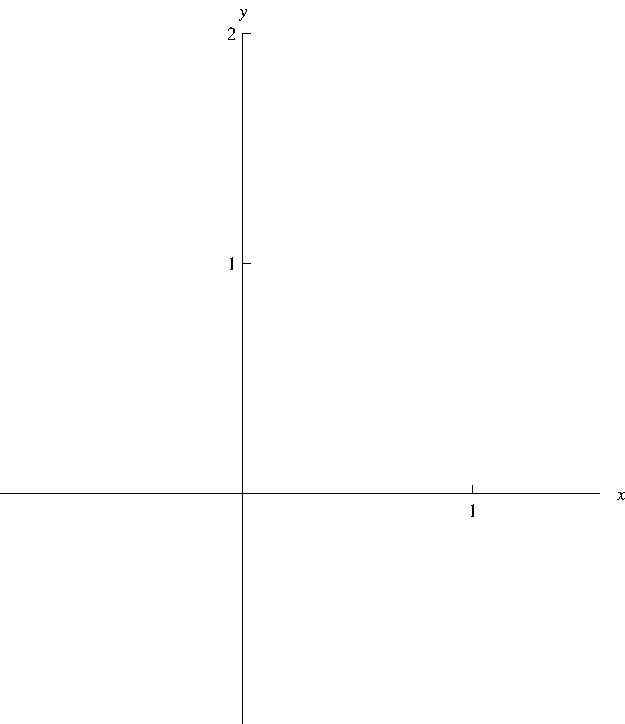
\includegraphics[height=4cm]{area-between-curves/pictures/06-01-ex2a.pdf}%
}%  
\only<handout:0| 6-7>{%
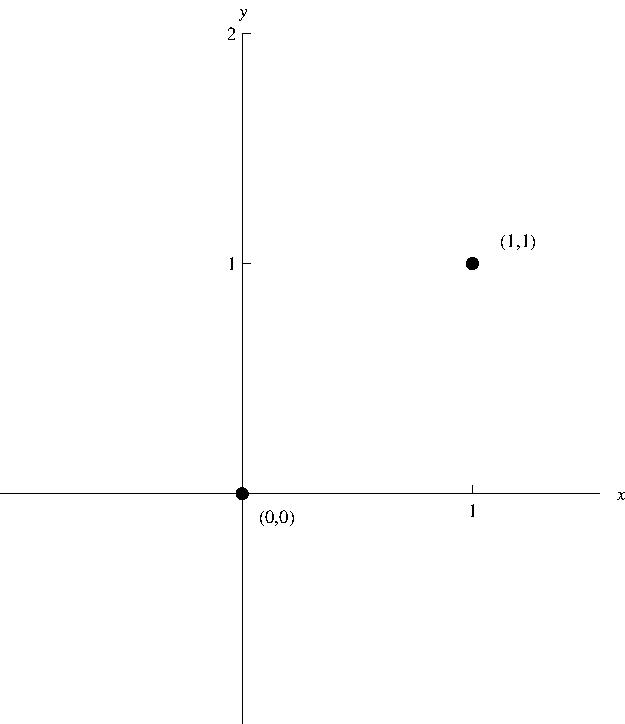
\includegraphics[height=4cm]{area-between-curves/pictures/06-01-ex2b.pdf}%
}%  
\only<handout:0| 8>{%
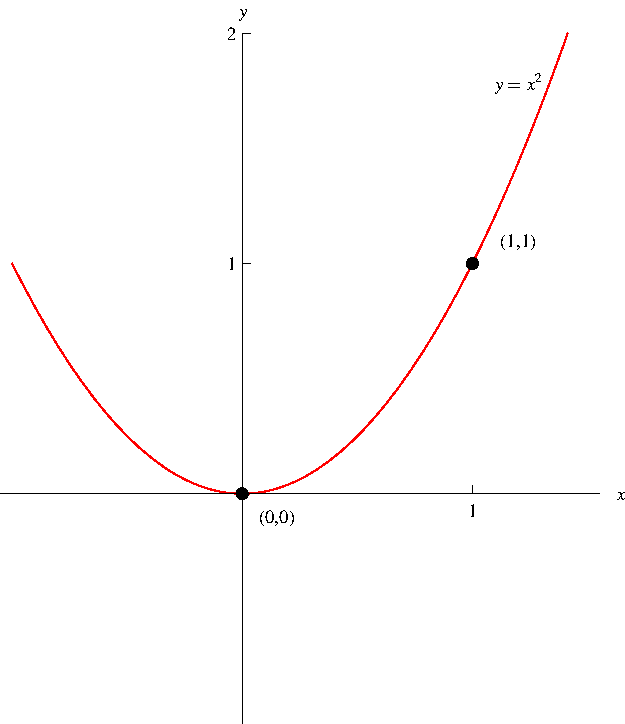
\includegraphics[height=4cm]{area-between-curves/pictures/06-01-ex2c.pdf}%
}%  
\only<handout:0| 9-10>{%
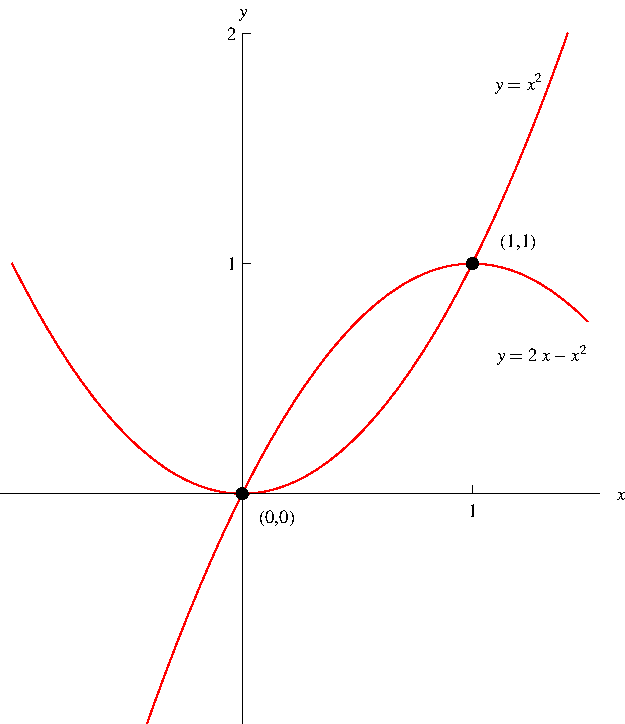
\includegraphics[height=4cm]{area-between-curves/pictures/06-01-ex2d.pdf}%
}%  
\only<11->{%
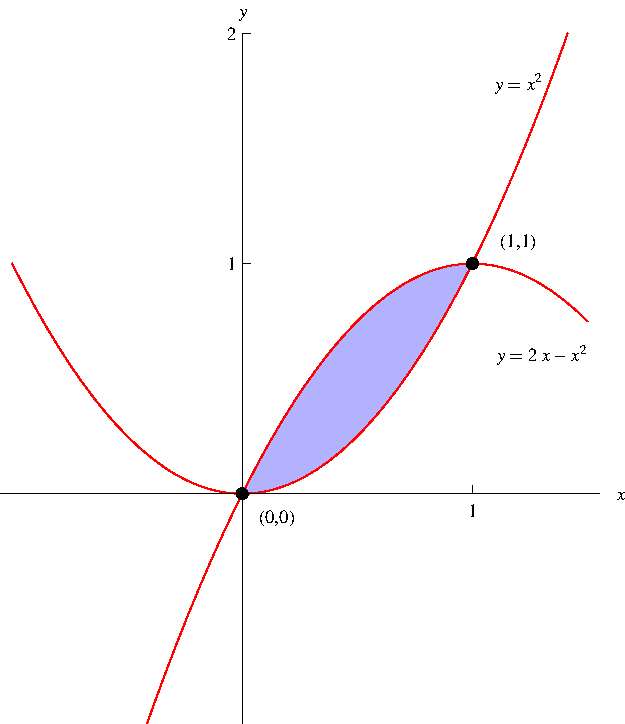
\includegraphics[height=4cm]{area-between-curves/pictures/06-01-ex2e.pdf}%
}%  
\begin{enumerate}
\item<2->  Find the point of intersection.
\item<7->  Graph the functions.
\item<10->  Identify the region.
\item<12->  Integrate.
\end{enumerate}

\column{.65\textwidth}
Find the area of the region enclosed by the parabolas $\alert<handout:0| 8>{y =} \alert<handout:0| 3,8>{x^2}$ and $\alert<handout:0| 9>{y =} \alert<handout:0| 3,9>{2x - x^2}$.
\begin{eqnarray*}
\uncover<3->{\alert<handout:0| 3>{x^2}} & \uncover<3->{\alert<handout:0| 3>{=}} & \uncover<3->{\alert<handout:0| 3>{2x - x^2}} \\
\uncover<4->{0} & \uncover<4->{=} & \uncover<4->{2x - 2x^2} \uncover<5->{ = 2x(1 - x)} \\
\uncover<6->{x} & \uncover<6->{=} & \uncover<6->{0 \textrm{ or } 1.}
\end{eqnarray*}
\begin{eqnarray*}
\uncover<13->{A} & \uncover<13->{=} & \uncover<13->{\int_0^1 (2x - 2x^2) \diff x} \uncover<14->{ = 2\int_0^1 (x - x^2) \diff x} \\
 & \uncover<15->{=} & \uncover<15->{2\left[ \frac{x^2}{2} - \frac{x^3}{3}\right]_0^1} \uncover<16->{ = 2\left( \frac{1}{2} - \frac{1}{3}\right)} \uncover<17->{ = \frac{1}{3}}
\end{eqnarray*}
\end{columns}
\end{example}
\end{frame}
% end module area-between-curves-ex2
